\documentclass[12pt]{article}
\usepackage[pdftex]{graphicx}
\usepackage{amsfonts}
\usepackage[italian]{babel}
\usepackage{graphicx}
\usepackage{color}
\usepackage{multirow,bigdelim}

\definecolor{grey}{rgb}{0.3,0.3,0.3}

\usepackage{listings, framed}
\lstset{
  language=Java,
  showstringspaces=false,
  columns=flexible,
  basicstyle={\small\ttfamily},
  frame=none,
  numbers=none,
  keywordstyle=\bfseries\color{grey},
  commentstyle=\itshape\color{red},
  identifierstyle=\color{black},
  stringstyle=\color{blue},
  numberstyle={\ttfamily},
%  breaklines=true,
  breakatwhitespace=true,
  tabsize=3,
  escapechar=|
}

%****************enlarge layout
\textheight     243.5mm
\topmargin      -20.0mm
\textwidth      480pt
\hoffset        -80pt
%*****************theorems and such
\newcounter{esnu}
\newenvironment{esercizio}{\medskip \noindent {\bf Esercizio\addtocounter{esnu}{1} \arabic{esnu}}}{}
\pagestyle{empty}
\newcommand{\liff}{\mathrel{\leftrightarrow}}   % Logical IFF Symbol
\newcommand{\metaiff}{\Longleftrightarrow}      %iff in metatheory

\begin{document}

%\begin{tabular}{llclcr}
% \hspace{-35pt} &{\bf COGNOME:} & \hspace{100pt}        &{\bf NOME:}    & \hspace{100pt}        &{\bf MATRICOLA:}%\hspace{35pt} \\
%\hline
%\end{tabular}
\begin{center} {\bf Esame di Programmazione II, 25 luglio 2019}\end{center}
%\`

\emph{
Si crei un progetto Eclipse e, nella directory dei sorgenti,
si crei il package \texttt{it.univr.words}. Si copi al suo interno
la classe \texttt{Words.java}. Si copi dentro il package di default la classe
\texttt{Main.java}. Si copino al livello base del progetto i tre file di testo
\texttt{1984.txt}, \texttt{animal\_farm.txt} e \texttt{try\_this.txt} (quest'ultimo lo
dovete generare voi con il comando \texttt{touch try\_this.txt}).
Il risultato dovrebbe quindi essere come nella figura seguente:}

\begin{center}
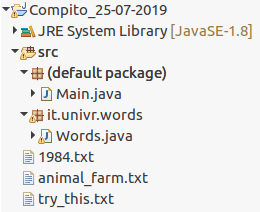
\includegraphics[width=8cm]{project.png}
\end{center}

\emph{
Se si realizzano nuove classi, le si crei dentro
il package \texttt{it.univr.words}.
Non si modifichi le dichiarazioni dei metodi. Si possono definire altri campi,
metodi, costruttori e classi, ma devono essere \texttt{private}.
La consegna fornita compila.
Anche la soluzione che verr\`a consegnata dovr\`a compilare,
altrimenti non verr\`a corretta.
}
\mbox{}\\

\begin{esercizio}~\textbf{[18 punti, si consegni \texttt{Words.java}]}
  Si completi la classe \texttt{Words.java}, che implementa una lista di parole
  lette da un file di testo, modificandola dove indicato con \texttt{TODO}.
  Quando un oggetto \texttt{Words} viene creato, esso
  deve accedere al file di testo
  indicato per nome, leggerlo parola per parola e aggiungere tali parole
  a se stesso (\texttt{this}). Le modifiche sono le seguenti:
  %
  \begin{enumerate}
  \item si faccia estendere a tale classe una classe della libreria Java
    standard che rappresenta liste di stringhe;
  \item si completino i due costruttori, che estraggono le parole
    di un file di testo e le aggiungono alla lista \texttt{this}. Si noti che
    i due costruttori si differenziano solo perch\'e il primo estrae
    tutte le parole, mentre il secondo estrae solo quelle che soddisfano
    un predicato estrattore. Il tipo per il predicato
    esiste gi\`a nella libreria
    standard ed \`e definito come segue:
    \begin{lstlisting}
    public interface java.util.function.Predicate<T> {
      boolean test(T t);  // controlla se t soddisfa il test
    }
    \end{lstlisting}
    I due costruttori devono lanciare una
    \texttt{IOException} (della libreria standard) se ci fosse
    un problema di accesso al file;
  \item si ridefinisca il metodo \texttt{toString()} in modo da ritornare
    una stringa del tipo \texttt{a list of XX words}, dove \texttt{XX} \`e
    la lunghezza della lista;
  \item si scriva il metodo \texttt{mostFrequent()} che restituisce la
    parola pi\`u frequente fra quelle contenute nella lista
    (in caso di parit\`a, restituisce la prima fra le pi\`u frequenti).
    Si noti che, se la lista fosse vuota, questo metodo dovr\`a
    lanciare una \texttt{NoSuchElementException}, la cui classe \`e nella
    libreria standard.
  \end{enumerate}
  \textbf{Suggerimenti:} Per leggere un file di testo si crei un
  oggetto lettore bufferizzato, in questo modo:
  \texttt{new BufferedReader(new FileReader(fileName))}.
  Chiamando ripetutamente su tale oggetto il metodo
  \texttt{readLine()}, si ottiene una riga (cio\`e una stringa)
  alla volta del file di
  testo e alla fine si ottiene \texttt{null} per segnalare la fine del file.
  Ogni riga pu\`o essere divisa in parole, scartando spaziatura e
  punteggiatura, usando il metodo delle stringhe
  \verb!split("\\W+")!.
  Non ci si dimentichi di chiudere il \texttt{BufferedReader}
  alla fine dell'utilizzo.
\end{esercizio}

\begin{esercizio}~\textbf{[14 punti, si consegni \texttt{Main.java}]}
  Si completi la classe \texttt{Main.java} in modo tale che la sua esecuzione:
  \begin{enumerate}
  \item chieda all'utente di inserire da tastiera il nome del file di testo da
    processare;
  \item crei un oggetto \texttt{Words} a partire da tale file, stampi a video
    tale oggetto e quindi stampi a video la sua parola pi\`u frequente;
  \item crei un oggetto \texttt{Words} a partire da tale file, selezionando solo le
    parole che cominciano con il carattere \texttt{J} (maiuscolo), stampi
    a video tale oggetto e quindi stampi a video la sua parola pi\`u frequente;
  \item crei un oggetto \texttt{Words} a partire da tale file, selezionando solo le
    parole che siano pi\`u lunghe di quattro caratteri, stampi
    a video tale oggetto e quindi stampi a video la sua parola pi\`u frequente;
  \item se la creazione di uno di questi tre \texttt{Words} fallisse
    con un'eccezione
    perch\'e non si riesce ad accedere al file, il \texttt{Main}
    dovr\`a stampare \texttt{There was a problem accessing FILENAME}
    e terminare;
  \item se una delle tre chiamate a \texttt{mostFrequent()} fallisse
    con un'eccezione perch\'e un oggetto \texttt{Words} \`e vuoto e quindi
    non ha un elemento pi\`u frequente, il \texttt{Main} dovr\`a
    stampare \texttt{I have selected zero words} e terminare.
  \end{enumerate}
\end{esercizio}

\mbox{}\\

\emph{Se tutto \`e  corretto, un'esecuzione del \texttt{Main}
  sul file di prova \texttt{1984.txt} dovrebbe rassomigliare a quanto segue:}
\begin{verbatim}
File name: 1984.txt

I have extracted a list of 107799 words
The most frequent word is "the"

I have extracted a list of 153 words that start with J
The most frequent word is "Julia"

I have extracted a list of 39910 words that are longer than four characters
The most frequent word is "Winston"
\end{verbatim}

\emph{Lo si provi anche con \texttt{animal\_farm.txt} e \texttt{try\_this.txt}.}

\end{document}
